% Created by tikzDevice version 0.10.1 on 2017-11-29 19:14:47
% !TEX encoding = UTF-8 Unicode
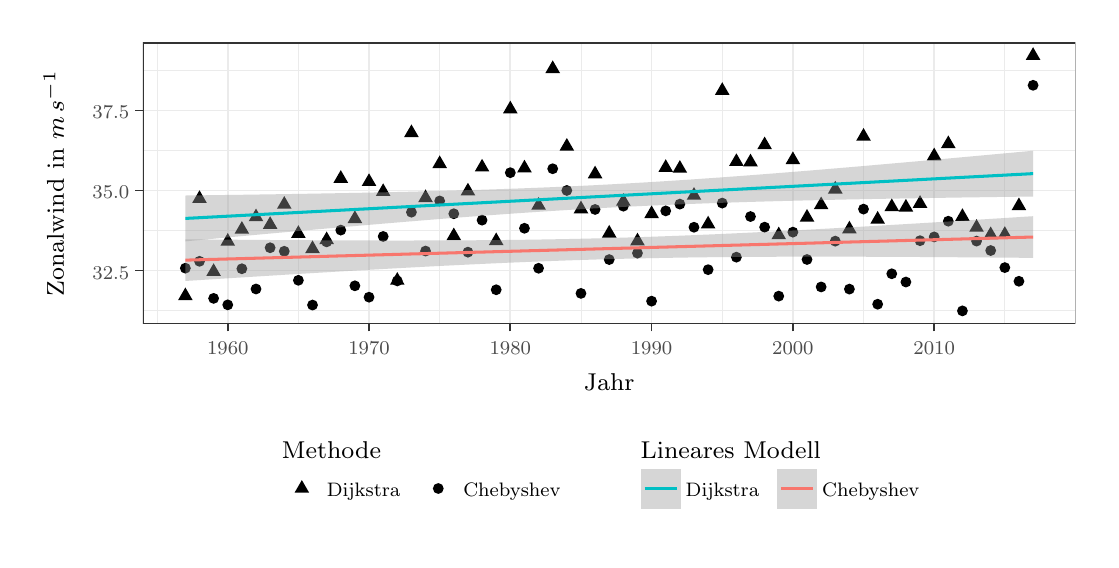
\begin{tikzpicture}[font=\footnotesize,x=1pt,y=1pt]
\definecolor{fillColor}{RGB}{255,255,255}
\path[use as bounding box,fill=fillColor,fill opacity=0.00] (0,0) rectangle (384.11,184.94);
\begin{scope}
\path[clip] (  0.00,  0.00) rectangle (384.11,184.94);
\definecolor{drawColor}{RGB}{255,255,255}
\definecolor{fillColor}{RGB}{255,255,255}

\path[draw=drawColor,line width= 0.6pt,line join=round,line cap=round,fill=fillColor] (  0.00,  0.00) rectangle (384.11,184.94);
\end{scope}
\begin{scope}
\path[clip] ( 41.67, 77.99) rectangle (378.61,179.44);
\definecolor{fillColor}{RGB}{255,255,255}

\path[fill=fillColor] ( 41.67, 77.99) rectangle (378.61,179.44);
\definecolor{drawColor}{gray}{0.92}

\path[draw=drawColor,line width= 0.3pt,line join=round] ( 41.67, 82.67) --
	(378.61, 82.67);

\path[draw=drawColor,line width= 0.3pt,line join=round] ( 41.67,111.60) --
	(378.61,111.60);

\path[draw=drawColor,line width= 0.3pt,line join=round] ( 41.67,140.53) --
	(378.61,140.53);

\path[draw=drawColor,line width= 0.3pt,line join=round] ( 41.67,169.46) --
	(378.61,169.46);

\path[draw=drawColor,line width= 0.3pt,line join=round] ( 46.77, 77.99) --
	( 46.77,179.44);

\path[draw=drawColor,line width= 0.3pt,line join=round] ( 97.82, 77.99) --
	( 97.82,179.44);

\path[draw=drawColor,line width= 0.3pt,line join=round] (148.88, 77.99) --
	(148.88,179.44);

\path[draw=drawColor,line width= 0.3pt,line join=round] (199.93, 77.99) --
	(199.93,179.44);

\path[draw=drawColor,line width= 0.3pt,line join=round] (250.98, 77.99) --
	(250.98,179.44);

\path[draw=drawColor,line width= 0.3pt,line join=round] (302.03, 77.99) --
	(302.03,179.44);

\path[draw=drawColor,line width= 0.3pt,line join=round] (353.09, 77.99) --
	(353.09,179.44);

\path[draw=drawColor,line width= 0.3pt,line join=round] (378.61, 77.99) --
	(378.61,179.44);

\path[draw=drawColor,line width= 0.6pt,line join=round] ( 41.67, 97.14) --
	(378.61, 97.14);

\path[draw=drawColor,line width= 0.6pt,line join=round] ( 41.67,126.07) --
	(378.61,126.07);

\path[draw=drawColor,line width= 0.6pt,line join=round] ( 41.67,154.99) --
	(378.61,154.99);

\path[draw=drawColor,line width= 0.6pt,line join=round] ( 72.30, 77.99) --
	( 72.30,179.44);

\path[draw=drawColor,line width= 0.6pt,line join=round] (123.35, 77.99) --
	(123.35,179.44);

\path[draw=drawColor,line width= 0.6pt,line join=round] (174.40, 77.99) --
	(174.40,179.44);

\path[draw=drawColor,line width= 0.6pt,line join=round] (225.45, 77.99) --
	(225.45,179.44);

\path[draw=drawColor,line width= 0.6pt,line join=round] (276.51, 77.99) --
	(276.51,179.44);

\path[draw=drawColor,line width= 0.6pt,line join=round] (327.56, 77.99) --
	(327.56,179.44);
\definecolor{fillColor}{RGB}{0,0,0}

\path[fill=fillColor] ( 56.98, 98.03) circle (  1.96);

\path[fill=fillColor] ( 62.09,100.51) circle (  1.96);

\path[fill=fillColor] ( 67.19, 87.12) circle (  1.96);

\path[fill=fillColor] ( 72.30, 84.78) circle (  1.96);

\path[fill=fillColor] ( 77.40, 97.82) circle (  1.96);

\path[fill=fillColor] ( 82.51, 90.51) circle (  1.96);

\path[fill=fillColor] ( 87.61,105.41) circle (  1.96);

\path[fill=fillColor] ( 92.72,104.14) circle (  1.96);

\path[fill=fillColor] ( 97.82, 93.65) circle (  1.96);

\path[fill=fillColor] (102.93, 84.71) circle (  1.96);

\path[fill=fillColor] (108.03,107.54) circle (  1.96);

\path[fill=fillColor] (113.14,111.79) circle (  1.96);

\path[fill=fillColor] (118.24, 91.66) circle (  1.96);

\path[fill=fillColor] (123.35, 87.55) circle (  1.96);

\path[fill=fillColor] (128.46,109.50) circle (  1.96);

\path[fill=fillColor] (133.56, 93.43) circle (  1.96);

\path[fill=fillColor] (138.67,118.26) circle (  1.96);

\path[fill=fillColor] (143.77,104.22) circle (  1.96);

\path[fill=fillColor] (148.88,122.32) circle (  1.96);

\path[fill=fillColor] (153.98,117.70) circle (  1.96);

\path[fill=fillColor] (159.09,103.82) circle (  1.96);

\path[fill=fillColor] (164.19,115.39) circle (  1.96);

\path[fill=fillColor] (169.30, 90.23) circle (  1.96);

\path[fill=fillColor] (174.40,132.54) circle (  1.96);

\path[fill=fillColor] (179.51,112.45) circle (  1.96);

\path[fill=fillColor] (184.61, 98.00) circle (  1.96);

\path[fill=fillColor] (189.72,133.96) circle (  1.96);

\path[fill=fillColor] (194.82,126.11) circle (  1.96);

\path[fill=fillColor] (199.93, 88.92) circle (  1.96);

\path[fill=fillColor] (205.03,119.25) circle (  1.96);

\path[fill=fillColor] (210.14,101.14) circle (  1.96);

\path[fill=fillColor] (215.24,120.44) circle (  1.96);

\path[fill=fillColor] (220.35,103.47) circle (  1.96);

\path[fill=fillColor] (225.45, 86.12) circle (  1.96);

\path[fill=fillColor] (230.56,118.73) circle (  1.96);

\path[fill=fillColor] (235.67,121.18) circle (  1.96);

\path[fill=fillColor] (240.77,112.82) circle (  1.96);

\path[fill=fillColor] (245.88, 97.49) circle (  1.96);

\path[fill=fillColor] (250.98,121.55) circle (  1.96);

\path[fill=fillColor] (256.09,102.01) circle (  1.96);

\path[fill=fillColor] (261.19,116.69) circle (  1.96);

\path[fill=fillColor] (266.30,112.86) circle (  1.96);

\path[fill=fillColor] (271.40, 87.93) circle (  1.96);

\path[fill=fillColor] (276.51,111.05) circle (  1.96);

\path[fill=fillColor] (281.61,101.17) circle (  1.96);

\path[fill=fillColor] (286.72, 91.25) circle (  1.96);

\path[fill=fillColor] (291.82,107.80) circle (  1.96);

\path[fill=fillColor] (296.93, 90.47) circle (  1.96);

\path[fill=fillColor] (302.03,119.38) circle (  1.96);

\path[fill=fillColor] (307.14, 85.01) circle (  1.96);

\path[fill=fillColor] (312.24, 96.01) circle (  1.96);

\path[fill=fillColor] (317.35, 93.03) circle (  1.96);

\path[fill=fillColor] (322.45,107.96) circle (  1.96);

\path[fill=fillColor] (327.56,109.33) circle (  1.96);

\path[fill=fillColor] (332.67,115.01) circle (  1.96);

\path[fill=fillColor] (337.77, 82.60) circle (  1.96);

\path[fill=fillColor] (342.88,107.82) circle (  1.96);

\path[fill=fillColor] (347.98,104.41) circle (  1.96);

\path[fill=fillColor] (353.09, 98.24) circle (  1.96);

\path[fill=fillColor] (358.19, 93.30) circle (  1.96);

\path[fill=fillColor] (363.30,164.12) circle (  1.96);

\path[fill=fillColor] ( 56.98, 91.06) --
	( 59.62, 86.48) --
	( 54.34, 86.48) --
	cycle;

\path[fill=fillColor] ( 62.09,126.19) --
	( 64.73,121.61) --
	( 59.44,121.61) --
	cycle;

\path[fill=fillColor] ( 67.19, 99.81) --
	( 69.83, 95.23) --
	( 64.55, 95.23) --
	cycle;

\path[fill=fillColor] ( 72.30,110.74) --
	( 74.94,106.16) --
	( 69.65,106.16) --
	cycle;

\path[fill=fillColor] ( 77.40,115.06) --
	( 80.05,110.48) --
	( 74.76,110.48) --
	cycle;

\path[fill=fillColor] ( 82.51,119.57) --
	( 85.15,114.99) --
	( 79.87,114.99) --
	cycle;

\path[fill=fillColor] ( 87.61,116.81) --
	( 90.26,112.23) --
	( 84.97,112.23) --
	cycle;

\path[fill=fillColor] ( 92.72,124.09) --
	( 95.36,119.51) --
	( 90.08,119.51) --
	cycle;

\path[fill=fillColor] ( 97.82,113.56) --
	(100.47,108.98) --
	( 95.18,108.98) --
	cycle;

\path[fill=fillColor] (102.93,108.07) --
	(105.57,103.50) --
	(100.29,103.50) --
	cycle;

\path[fill=fillColor] (108.03,111.30) --
	(110.68,106.72) --
	(105.39,106.72) --
	cycle;

\path[fill=fillColor] (113.14,133.47) --
	(115.78,128.90) --
	(110.50,128.90) --
	cycle;

\path[fill=fillColor] (118.24,118.93) --
	(120.89,114.35) --
	(115.60,114.35) --
	cycle;

\path[fill=fillColor] (123.35,132.32) --
	(125.99,127.75) --
	(120.71,127.75) --
	cycle;

\path[fill=fillColor] (128.46,128.70) --
	(131.10,124.12) --
	(125.81,124.12) --
	cycle;

\path[fill=fillColor] (133.56, 96.63) --
	(136.20, 92.06) --
	(130.92, 92.06) --
	cycle;

\path[fill=fillColor] (138.67,149.98) --
	(141.31,145.41) --
	(136.02,145.41) --
	cycle;

\path[fill=fillColor] (143.77,126.50) --
	(146.41,121.92) --
	(141.13,121.92) --
	cycle;

\path[fill=fillColor] (148.88,138.79) --
	(151.52,134.21) --
	(146.23,134.21) --
	cycle;

\path[fill=fillColor] (153.98,112.73) --
	(156.62,108.16) --
	(151.34,108.16) --
	cycle;

\path[fill=fillColor] (159.09,128.90) --
	(161.73,124.33) --
	(156.44,124.33) --
	cycle;

\path[fill=fillColor] (164.19,137.55) --
	(166.83,132.97) --
	(161.55,132.97) --
	cycle;

\path[fill=fillColor] (169.30,110.94) --
	(171.94,106.37) --
	(166.65,106.37) --
	cycle;

\path[fill=fillColor] (174.40,158.56) --
	(177.04,153.98) --
	(171.76,153.98) --
	cycle;

\path[fill=fillColor] (179.51,137.23) --
	(182.15,132.65) --
	(176.87,132.65) --
	cycle;

\path[fill=fillColor] (184.61,123.76) --
	(187.26,119.18) --
	(181.97,119.18) --
	cycle;

\path[fill=fillColor] (189.72,173.12) --
	(192.36,168.55) --
	(187.08,168.55) --
	cycle;

\path[fill=fillColor] (194.82,145.07) --
	(197.47,140.50) --
	(192.18,140.50) --
	cycle;

\path[fill=fillColor] (199.93,122.45) --
	(202.57,117.87) --
	(197.29,117.87) --
	cycle;

\path[fill=fillColor] (205.03,135.09) --
	(207.68,130.52) --
	(202.39,130.52) --
	cycle;

\path[fill=fillColor] (210.14,113.68) --
	(212.78,109.10) --
	(207.50,109.10) --
	cycle;

\path[fill=fillColor] (215.24,125.17) --
	(217.89,120.60) --
	(212.60,120.60) --
	cycle;

\path[fill=fillColor] (220.35,110.86) --
	(222.99,106.28) --
	(217.71,106.28) --
	cycle;

\path[fill=fillColor] (225.45,120.71) --
	(228.10,116.14) --
	(222.81,116.14) --
	cycle;

\path[fill=fillColor] (230.56,137.41) --
	(233.20,132.83) --
	(227.92,132.83) --
	cycle;

\path[fill=fillColor] (235.67,137.09) --
	(238.31,132.52) --
	(233.02,132.52) --
	cycle;

\path[fill=fillColor] (240.77,127.33) --
	(243.41,122.76) --
	(238.13,122.76) --
	cycle;

\path[fill=fillColor] (245.88,116.98) --
	(248.52,112.41) --
	(243.23,112.41) --
	cycle;

\path[fill=fillColor] (250.98,165.23) --
	(253.62,160.65) --
	(248.34,160.65) --
	cycle;

\path[fill=fillColor] (256.09,139.54) --
	(258.73,134.97) --
	(253.44,134.97) --
	cycle;

\path[fill=fillColor] (261.19,139.41) --
	(263.83,134.84) --
	(258.55,134.84) --
	cycle;

\path[fill=fillColor] (266.30,145.60) --
	(268.94,141.03) --
	(263.65,141.03) --
	cycle;

\path[fill=fillColor] (271.40,113.06) --
	(274.04,108.49) --
	(268.76,108.49) --
	cycle;

\path[fill=fillColor] (276.51,140.22) --
	(279.15,135.64) --
	(273.86,135.64) --
	cycle;

\path[fill=fillColor] (281.61,119.42) --
	(284.26,114.85) --
	(278.97,114.85) --
	cycle;

\path[fill=fillColor] (286.72,123.92) --
	(289.36,119.35) --
	(284.08,119.35) --
	cycle;

\path[fill=fillColor] (291.82,129.59) --
	(294.47,125.01) --
	(289.18,125.01) --
	cycle;

\path[fill=fillColor] (296.93,115.19) --
	(299.57,110.61) --
	(294.29,110.61) --
	cycle;

\path[fill=fillColor] (302.03,148.69) --
	(304.68,144.11) --
	(299.39,144.11) --
	cycle;

\path[fill=fillColor] (307.14,118.71) --
	(309.78,114.13) --
	(304.50,114.13) --
	cycle;

\path[fill=fillColor] (312.24,123.24) --
	(314.89,118.67) --
	(309.60,118.67) --
	cycle;

\path[fill=fillColor] (317.35,123.07) --
	(319.99,118.50) --
	(314.71,118.50) --
	cycle;

\path[fill=fillColor] (322.45,124.43) --
	(325.10,119.85) --
	(319.81,119.85) --
	cycle;

\path[fill=fillColor] (327.56,141.60) --
	(330.20,137.03) --
	(324.92,137.03) --
	cycle;

\path[fill=fillColor] (332.67,146.00) --
	(335.31,141.42) --
	(330.02,141.42) --
	cycle;

\path[fill=fillColor] (337.77,119.69) --
	(340.41,115.11) --
	(335.13,115.11) --
	cycle;

\path[fill=fillColor] (342.88,115.77) --
	(345.52,111.20) --
	(340.23,111.20) --
	cycle;

\path[fill=fillColor] (347.98,113.11) --
	(350.62,108.53) --
	(345.34,108.53) --
	cycle;

\path[fill=fillColor] (353.09,113.20) --
	(355.73,108.62) --
	(350.44,108.62) --
	cycle;

\path[fill=fillColor] (358.19,123.60) --
	(360.83,119.03) --
	(355.55,119.03) --
	cycle;

\path[fill=fillColor] (363.30,177.88) --
	(365.94,173.31) --
	(360.65,173.31) --
	cycle;
\definecolor{fillColor}{RGB}{153,153,153}

\path[fill=fillColor,fill opacity=0.40] ( 56.98,108.47) --
	( 60.86,108.43) --
	( 64.74,108.40) --
	( 68.61,108.36) --
	( 72.49,108.33) --
	( 76.37,108.30) --
	( 80.25,108.27) --
	( 84.12,108.24) --
	( 88.00,108.21) --
	( 91.88,108.19) --
	( 95.76,108.16) --
	( 99.63,108.14) --
	(103.51,108.12) --
	(107.39,108.10) --
	(111.27,108.08) --
	(115.14,108.07) --
	(119.02,108.05) --
	(122.90,108.04) --
	(126.78,108.04) --
	(130.65,108.03) --
	(134.53,108.03) --
	(138.41,108.03) --
	(142.28,108.04) --
	(146.16,108.04) --
	(150.04,108.06) --
	(153.92,108.07) --
	(157.79,108.09) --
	(161.67,108.12) --
	(165.55,108.15) --
	(169.43,108.18) --
	(173.30,108.22) --
	(177.18,108.27) --
	(181.06,108.32) --
	(184.94,108.38) --
	(188.81,108.45) --
	(192.69,108.52) --
	(196.57,108.59) --
	(200.45,108.68) --
	(204.32,108.77) --
	(208.20,108.87) --
	(212.08,108.97) --
	(215.96,109.09) --
	(219.83,109.21) --
	(223.71,109.33) --
	(227.59,109.47) --
	(231.46,109.61) --
	(235.34,109.75) --
	(239.22,109.91) --
	(243.10,110.07) --
	(246.97,110.23) --
	(250.85,110.40) --
	(254.73,110.58) --
	(258.61,110.76) --
	(262.48,110.95) --
	(266.36,111.14) --
	(270.24,111.33) --
	(274.12,111.53) --
	(277.99,111.73) --
	(281.87,111.94) --
	(285.75,112.15) --
	(289.63,112.36) --
	(293.50,112.58) --
	(297.38,112.80) --
	(301.26,113.02) --
	(305.14,113.24) --
	(309.01,113.47) --
	(312.89,113.70) --
	(316.77,113.93) --
	(320.65,114.16) --
	(324.52,114.39) --
	(328.40,114.63) --
	(332.28,114.87) --
	(336.15,115.11) --
	(340.03,115.35) --
	(343.91,115.59) --
	(347.79,115.83) --
	(351.66,116.07) --
	(355.54,116.32) --
	(359.42,116.57) --
	(363.30,116.81) --
	(363.30,101.75) --
	(359.42,101.79) --
	(355.54,101.82) --
	(351.66,101.86) --
	(347.79,101.89) --
	(343.91,101.92) --
	(340.03,101.95) --
	(336.15,101.98) --
	(332.28,102.01) --
	(328.40,102.03) --
	(324.52,102.06) --
	(320.65,102.08) --
	(316.77,102.10) --
	(312.89,102.12) --
	(309.01,102.14) --
	(305.14,102.15) --
	(301.26,102.17) --
	(297.38,102.18) --
	(293.50,102.18) --
	(289.63,102.19) --
	(285.75,102.19) --
	(281.87,102.19) --
	(277.99,102.18) --
	(274.12,102.18) --
	(270.24,102.16) --
	(266.36,102.15) --
	(262.48,102.13) --
	(258.61,102.10) --
	(254.73,102.07) --
	(250.85,102.04) --
	(246.97,102.00) --
	(243.10,101.95) --
	(239.22,101.90) --
	(235.34,101.84) --
	(231.46,101.77) --
	(227.59,101.70) --
	(223.71,101.63) --
	(219.83,101.54) --
	(215.96,101.45) --
	(212.08,101.35) --
	(208.20,101.25) --
	(204.32,101.13) --
	(200.45,101.01) --
	(196.57,100.89) --
	(192.69,100.75) --
	(188.81,100.61) --
	(184.94,100.47) --
	(181.06,100.31) --
	(177.18,100.15) --
	(173.30, 99.99) --
	(169.43, 99.82) --
	(165.55, 99.64) --
	(161.67, 99.46) --
	(157.79, 99.27) --
	(153.92, 99.08) --
	(150.04, 98.89) --
	(146.16, 98.69) --
	(142.28, 98.49) --
	(138.41, 98.28) --
	(134.53, 98.07) --
	(130.65, 97.86) --
	(126.78, 97.64) --
	(122.90, 97.42) --
	(119.02, 97.20) --
	(115.14, 96.98) --
	(111.27, 96.75) --
	(107.39, 96.52) --
	(103.51, 96.29) --
	( 99.63, 96.06) --
	( 95.76, 95.83) --
	( 91.88, 95.59) --
	( 88.00, 95.35) --
	( 84.12, 95.11) --
	( 80.25, 94.87) --
	( 76.37, 94.63) --
	( 72.49, 94.39) --
	( 68.61, 94.15) --
	( 64.74, 93.90) --
	( 60.86, 93.65) --
	( 56.98, 93.41) --
	cycle;
\definecolor{drawColor}{RGB}{248,118,109}

\path[draw=drawColor,line width= 1.1pt,line join=round] ( 56.98,100.94) --
	( 60.86,101.04) --
	( 64.74,101.15) --
	( 68.61,101.25) --
	( 72.49,101.36) --
	( 76.37,101.46) --
	( 80.25,101.57) --
	( 84.12,101.68) --
	( 88.00,101.78) --
	( 91.88,101.89) --
	( 95.76,101.99) --
	( 99.63,102.10) --
	(103.51,102.20) --
	(107.39,102.31) --
	(111.27,102.42) --
	(115.14,102.52) --
	(119.02,102.63) --
	(122.90,102.73) --
	(126.78,102.84) --
	(130.65,102.94) --
	(134.53,103.05) --
	(138.41,103.16) --
	(142.28,103.26) --
	(146.16,103.37) --
	(150.04,103.47) --
	(153.92,103.58) --
	(157.79,103.68) --
	(161.67,103.79) --
	(165.55,103.89) --
	(169.43,104.00) --
	(173.30,104.11) --
	(177.18,104.21) --
	(181.06,104.32) --
	(184.94,104.42) --
	(188.81,104.53) --
	(192.69,104.63) --
	(196.57,104.74) --
	(200.45,104.85) --
	(204.32,104.95) --
	(208.20,105.06) --
	(212.08,105.16) --
	(215.96,105.27) --
	(219.83,105.37) --
	(223.71,105.48) --
	(227.59,105.59) --
	(231.46,105.69) --
	(235.34,105.80) --
	(239.22,105.90) --
	(243.10,106.01) --
	(246.97,106.11) --
	(250.85,106.22) --
	(254.73,106.33) --
	(258.61,106.43) --
	(262.48,106.54) --
	(266.36,106.64) --
	(270.24,106.75) --
	(274.12,106.85) --
	(277.99,106.96) --
	(281.87,107.06) --
	(285.75,107.17) --
	(289.63,107.28) --
	(293.50,107.38) --
	(297.38,107.49) --
	(301.26,107.59) --
	(305.14,107.70) --
	(309.01,107.80) --
	(312.89,107.91) --
	(316.77,108.02) --
	(320.65,108.12) --
	(324.52,108.23) --
	(328.40,108.33) --
	(332.28,108.44) --
	(336.15,108.54) --
	(340.03,108.65) --
	(343.91,108.76) --
	(347.79,108.86) --
	(351.66,108.97) --
	(355.54,109.07) --
	(359.42,109.18) --
	(363.30,109.28);

\path[fill=fillColor,fill opacity=0.40] ( 56.98,124.29) --
	( 60.86,124.33) --
	( 64.74,124.39) --
	( 68.61,124.44) --
	( 72.49,124.49) --
	( 76.37,124.54) --
	( 80.25,124.60) --
	( 84.12,124.66) --
	( 88.00,124.72) --
	( 91.88,124.78) --
	( 95.76,124.84) --
	( 99.63,124.90) --
	(103.51,124.97) --
	(107.39,125.04) --
	(111.27,125.11) --
	(115.14,125.18) --
	(119.02,125.25) --
	(122.90,125.33) --
	(126.78,125.41) --
	(130.65,125.49) --
	(134.53,125.58) --
	(138.41,125.67) --
	(142.28,125.77) --
	(146.16,125.86) --
	(150.04,125.97) --
	(153.92,126.07) --
	(157.79,126.18) --
	(161.67,126.30) --
	(165.55,126.42) --
	(169.43,126.55) --
	(173.30,126.68) --
	(177.18,126.82) --
	(181.06,126.97) --
	(184.94,127.12) --
	(188.81,127.28) --
	(192.69,127.45) --
	(196.57,127.62) --
	(200.45,127.80) --
	(204.32,127.99) --
	(208.20,128.19) --
	(212.08,128.40) --
	(215.96,128.61) --
	(219.83,128.83) --
	(223.71,129.06) --
	(227.59,129.29) --
	(231.46,129.54) --
	(235.34,129.79) --
	(239.22,130.04) --
	(243.10,130.31) --
	(246.97,130.58) --
	(250.85,130.85) --
	(254.73,131.14) --
	(258.61,131.42) --
	(262.48,131.72) --
	(266.36,132.02) --
	(270.24,132.32) --
	(274.12,132.63) --
	(277.99,132.94) --
	(281.87,133.25) --
	(285.75,133.57) --
	(289.63,133.90) --
	(293.50,134.22) --
	(297.38,134.55) --
	(301.26,134.88) --
	(305.14,135.22) --
	(309.01,135.56) --
	(312.89,135.90) --
	(316.77,136.24) --
	(320.65,136.58) --
	(324.52,136.93) --
	(328.40,137.28) --
	(332.28,137.63) --
	(336.15,137.98) --
	(340.03,138.33) --
	(343.91,138.68) --
	(347.79,139.04) --
	(351.66,139.40) --
	(355.54,139.75) --
	(359.42,140.11) --
	(363.30,140.47) --
	(363.30,123.92) --
	(359.42,123.87) --
	(355.54,123.82) --
	(351.66,123.77) --
	(347.79,123.72) --
	(343.91,123.66) --
	(340.03,123.61) --
	(336.15,123.55) --
	(332.28,123.49) --
	(328.40,123.43) --
	(324.52,123.37) --
	(320.65,123.30) --
	(316.77,123.24) --
	(312.89,123.17) --
	(309.01,123.10) --
	(305.14,123.03) --
	(301.26,122.95) --
	(297.38,122.88) --
	(293.50,122.80) --
	(289.63,122.71) --
	(285.75,122.62) --
	(281.87,122.53) --
	(277.99,122.44) --
	(274.12,122.34) --
	(270.24,122.24) --
	(266.36,122.13) --
	(262.48,122.02) --
	(258.61,121.91) --
	(254.73,121.78) --
	(250.85,121.66) --
	(246.97,121.52) --
	(243.10,121.38) --
	(239.22,121.24) --
	(235.34,121.08) --
	(231.46,120.92) --
	(227.59,120.76) --
	(223.71,120.58) --
	(219.83,120.40) --
	(215.96,120.21) --
	(212.08,120.02) --
	(208.20,119.81) --
	(204.32,119.60) --
	(200.45,119.38) --
	(196.57,119.15) --
	(192.69,118.91) --
	(188.81,118.67) --
	(184.94,118.42) --
	(181.06,118.16) --
	(177.18,117.90) --
	(173.30,117.63) --
	(169.43,117.35) --
	(165.55,117.07) --
	(161.67,116.78) --
	(157.79,116.49) --
	(153.92,116.19) --
	(150.04,115.89) --
	(146.16,115.58) --
	(142.28,115.27) --
	(138.41,114.95) --
	(134.53,114.63) --
	(130.65,114.31) --
	(126.78,113.98) --
	(122.90,113.65) --
	(119.02,113.32) --
	(115.14,112.99) --
	(111.27,112.65) --
	(107.39,112.31) --
	(103.51,111.97) --
	( 99.63,111.62) --
	( 95.76,111.28) --
	( 91.88,110.93) --
	( 88.00,110.58) --
	( 84.12,110.23) --
	( 80.25,109.88) --
	( 76.37,109.52) --
	( 72.49,109.17) --
	( 68.61,108.81) --
	( 64.74,108.45) --
	( 60.86,108.09) --
	( 56.98,107.73) --
	cycle;
\definecolor{drawColor}{RGB}{0,191,196}

\path[draw=drawColor,line width= 1.1pt,line join=round] ( 56.98,116.01) --
	( 60.86,116.21) --
	( 64.74,116.42) --
	( 68.61,116.62) --
	( 72.49,116.83) --
	( 76.37,117.03) --
	( 80.25,117.24) --
	( 84.12,117.44) --
	( 88.00,117.65) --
	( 91.88,117.85) --
	( 95.76,118.06) --
	( 99.63,118.26) --
	(103.51,118.47) --
	(107.39,118.67) --
	(111.27,118.88) --
	(115.14,119.08) --
	(119.02,119.29) --
	(122.90,119.49) --
	(126.78,119.70) --
	(130.65,119.90) --
	(134.53,120.11) --
	(138.41,120.31) --
	(142.28,120.52) --
	(146.16,120.72) --
	(150.04,120.93) --
	(153.92,121.13) --
	(157.79,121.34) --
	(161.67,121.54) --
	(165.55,121.75) --
	(169.43,121.95) --
	(173.30,122.16) --
	(177.18,122.36) --
	(181.06,122.57) --
	(184.94,122.77) --
	(188.81,122.98) --
	(192.69,123.18) --
	(196.57,123.39) --
	(200.45,123.59) --
	(204.32,123.80) --
	(208.20,124.00) --
	(212.08,124.21) --
	(215.96,124.41) --
	(219.83,124.62) --
	(223.71,124.82) --
	(227.59,125.03) --
	(231.46,125.23) --
	(235.34,125.44) --
	(239.22,125.64) --
	(243.10,125.84) --
	(246.97,126.05) --
	(250.85,126.25) --
	(254.73,126.46) --
	(258.61,126.66) --
	(262.48,126.87) --
	(266.36,127.07) --
	(270.24,127.28) --
	(274.12,127.48) --
	(277.99,127.69) --
	(281.87,127.89) --
	(285.75,128.10) --
	(289.63,128.30) --
	(293.50,128.51) --
	(297.38,128.71) --
	(301.26,128.92) --
	(305.14,129.12) --
	(309.01,129.33) --
	(312.89,129.53) --
	(316.77,129.74) --
	(320.65,129.94) --
	(324.52,130.15) --
	(328.40,130.35) --
	(332.28,130.56) --
	(336.15,130.76) --
	(340.03,130.97) --
	(343.91,131.17) --
	(347.79,131.38) --
	(351.66,131.58) --
	(355.54,131.79) --
	(359.42,131.99) --
	(363.30,132.20);
\definecolor{drawColor}{gray}{0.20}

\path[draw=drawColor,line width= 0.6pt,line join=round,line cap=round] ( 41.67, 77.99) rectangle (378.61,179.44);
\end{scope}
\begin{scope}
\path[clip] (  0.00,  0.00) rectangle (384.11,184.94);
\definecolor{drawColor}{gray}{0.30}

\node[text=drawColor,anchor=base east,inner sep=0pt, outer sep=0pt, scale=  0.88] at ( 36.72, 94.11) {32.5};

\node[text=drawColor,anchor=base east,inner sep=0pt, outer sep=0pt, scale=  0.88] at ( 36.72,123.04) {35.0};

\node[text=drawColor,anchor=base east,inner sep=0pt, outer sep=0pt, scale=  0.88] at ( 36.72,151.96) {37.5};
\end{scope}
\begin{scope}
\path[clip] (  0.00,  0.00) rectangle (384.11,184.94);
\definecolor{drawColor}{gray}{0.20}

\path[draw=drawColor,line width= 0.6pt,line join=round] ( 38.92, 97.14) --
	( 41.67, 97.14);

\path[draw=drawColor,line width= 0.6pt,line join=round] ( 38.92,126.07) --
	( 41.67,126.07);

\path[draw=drawColor,line width= 0.6pt,line join=round] ( 38.92,154.99) --
	( 41.67,154.99);
\end{scope}
\begin{scope}
\path[clip] (  0.00,  0.00) rectangle (384.11,184.94);
\definecolor{drawColor}{gray}{0.20}

\path[draw=drawColor,line width= 0.6pt,line join=round] ( 72.30, 75.24) --
	( 72.30, 77.99);

\path[draw=drawColor,line width= 0.6pt,line join=round] (123.35, 75.24) --
	(123.35, 77.99);

\path[draw=drawColor,line width= 0.6pt,line join=round] (174.40, 75.24) --
	(174.40, 77.99);

\path[draw=drawColor,line width= 0.6pt,line join=round] (225.45, 75.24) --
	(225.45, 77.99);

\path[draw=drawColor,line width= 0.6pt,line join=round] (276.51, 75.24) --
	(276.51, 77.99);

\path[draw=drawColor,line width= 0.6pt,line join=round] (327.56, 75.24) --
	(327.56, 77.99);
\end{scope}
\begin{scope}
\path[clip] (  0.00,  0.00) rectangle (384.11,184.94);
\definecolor{drawColor}{gray}{0.30}

\node[text=drawColor,anchor=base,inner sep=0pt, outer sep=0pt, scale=  0.88] at ( 72.30, 66.98) {1960};

\node[text=drawColor,anchor=base,inner sep=0pt, outer sep=0pt, scale=  0.88] at (123.35, 66.98) {1970};

\node[text=drawColor,anchor=base,inner sep=0pt, outer sep=0pt, scale=  0.88] at (174.40, 66.98) {1980};

\node[text=drawColor,anchor=base,inner sep=0pt, outer sep=0pt, scale=  0.88] at (225.45, 66.98) {1990};

\node[text=drawColor,anchor=base,inner sep=0pt, outer sep=0pt, scale=  0.88] at (276.51, 66.98) {2000};

\node[text=drawColor,anchor=base,inner sep=0pt, outer sep=0pt, scale=  0.88] at (327.56, 66.98) {2010};
\end{scope}
\begin{scope}
\path[clip] (  0.00,  0.00) rectangle (384.11,184.94);
\definecolor{drawColor}{RGB}{0,0,0}

\node[text=drawColor,anchor=base,inner sep=0pt, outer sep=0pt, scale=  1.10] at (210.14, 53.91) {Jahr};
\end{scope}
\begin{scope}
\path[clip] (  0.00,  0.00) rectangle (384.11,184.94);
\definecolor{drawColor}{RGB}{0,0,0}

\node[text=drawColor,rotate= 90.00,anchor=base,inner sep=0pt, outer sep=0pt, scale=  1.10] at ( 13.08,128.72) {Zonalwind in $m\,s^{-1}$};
\end{scope}
\begin{scope}
\path[clip] (  0.00,  0.00) rectangle (384.11,184.94);
\definecolor{fillColor}{RGB}{255,255,255}

\path[fill=fillColor] ( 86.16,  5.50) rectangle (204.45, 42.52);
\end{scope}
\begin{scope}
\path[clip] (  0.00,  0.00) rectangle (384.11,184.94);
\definecolor{drawColor}{RGB}{0,0,0}

\node[text=drawColor,anchor=base west,inner sep=0pt, outer sep=0pt, scale=  1.10] at ( 91.85, 29.26) {Methode};
\end{scope}
\begin{scope}
\path[clip] (  0.00,  0.00) rectangle (384.11,184.94);
\definecolor{fillColor}{RGB}{255,255,255}

\path[fill=fillColor] ( 91.85, 11.19) rectangle (106.30, 25.64);
\end{scope}
\begin{scope}
\path[clip] (  0.00,  0.00) rectangle (384.11,184.94);
\definecolor{fillColor}{RGB}{0,0,0}

\path[fill=fillColor] ( 99.07, 21.47) --
	(101.72, 16.89) --
	( 96.43, 16.89) --
	cycle;
\end{scope}
\begin{scope}
\path[clip] (  0.00,  0.00) rectangle (384.11,184.94);
\definecolor{fillColor}{RGB}{255,255,255}

\path[fill=fillColor] (141.15, 11.19) rectangle (155.60, 25.64);
\end{scope}
\begin{scope}
\path[clip] (  0.00,  0.00) rectangle (384.11,184.94);
\definecolor{fillColor}{RGB}{0,0,0}

\path[fill=fillColor] (148.37, 18.42) circle (  1.96);
\end{scope}
\begin{scope}
\path[clip] (  0.00,  0.00) rectangle (384.11,184.94);
\definecolor{drawColor}{RGB}{0,0,0}

\node[text=drawColor,anchor=base west,inner sep=0pt, outer sep=0pt, scale=  0.88] at (108.11, 15.39) {Dijkstra};
\end{scope}
\begin{scope}
\path[clip] (  0.00,  0.00) rectangle (384.11,184.94);
\definecolor{drawColor}{RGB}{0,0,0}

\node[text=drawColor,anchor=base west,inner sep=0pt, outer sep=0pt, scale=  0.88] at (157.41, 15.39) {Chebyshev};
\end{scope}
\begin{scope}
\path[clip] (  0.00,  0.00) rectangle (384.11,184.94);
\definecolor{fillColor}{RGB}{255,255,255}

\path[fill=fillColor] (215.83,  5.50) rectangle (334.12, 42.52);
\end{scope}
\begin{scope}
\path[clip] (  0.00,  0.00) rectangle (384.11,184.94);
\definecolor{drawColor}{RGB}{0,0,0}

\node[text=drawColor,anchor=base west,inner sep=0pt, outer sep=0pt, scale=  1.10] at (221.52, 29.26) {Lineares Modell};
\end{scope}
\begin{scope}
\path[clip] (  0.00,  0.00) rectangle (384.11,184.94);
\definecolor{fillColor}{RGB}{255,255,255}

\path[fill=fillColor] (221.52, 11.19) rectangle (235.97, 25.64);
\end{scope}
\begin{scope}
\path[clip] (  0.00,  0.00) rectangle (384.11,184.94);
\definecolor{fillColor}{RGB}{153,153,153}

\path[fill=fillColor,fill opacity=0.40] (221.52, 11.19) rectangle (235.97, 25.64);
\definecolor{drawColor}{RGB}{0,191,196}

\path[draw=drawColor,line width= 1.1pt,line join=round] (222.97, 18.42) -- (234.53, 18.42);
\end{scope}
\begin{scope}
\path[clip] (  0.00,  0.00) rectangle (384.11,184.94);
\definecolor{fillColor}{RGB}{255,255,255}

\path[fill=fillColor] (270.82, 11.19) rectangle (285.27, 25.64);
\end{scope}
\begin{scope}
\path[clip] (  0.00,  0.00) rectangle (384.11,184.94);
\definecolor{fillColor}{RGB}{153,153,153}

\path[fill=fillColor,fill opacity=0.40] (270.82, 11.19) rectangle (285.27, 25.64);
\definecolor{drawColor}{RGB}{248,118,109}

\path[draw=drawColor,line width= 1.1pt,line join=round] (272.27, 18.42) -- (283.83, 18.42);
\end{scope}
\begin{scope}
\path[clip] (  0.00,  0.00) rectangle (384.11,184.94);
\definecolor{drawColor}{RGB}{0,0,0}

\node[text=drawColor,anchor=base west,inner sep=0pt, outer sep=0pt, scale=  0.88] at (237.78, 15.39) {Dijkstra};
\end{scope}
\begin{scope}
\path[clip] (  0.00,  0.00) rectangle (384.11,184.94);
\definecolor{drawColor}{RGB}{0,0,0}

\node[text=drawColor,anchor=base west,inner sep=0pt, outer sep=0pt, scale=  0.88] at (287.08, 15.39) {Chebyshev};
\end{scope}
\end{tikzpicture}
